% ─────────────────────────────────────────────────────────────────────────────
% AI Agent Lab — Educational Guide
% MCP + A2A + Groq in Django
% Sesame University 2025–2026
% ─────────────────────────────────────────────────────────────────────────────
\documentclass[11pt,a4paper]{article}

% ── Packages ──────────────────────────────────────────────────────────────────
\usepackage[utf8]{inputenc}
\usepackage[T1]{fontenc}
\usepackage[english]{babel}
\usepackage{geometry}
\geometry{margin=2.5cm, top=2.8cm, bottom=2.8cm}

\usepackage{lmodern}
\usepackage{microtype}
\usepackage{parskip}
\usepackage{setspace}
\usepackage{booktabs}
\usepackage{tabularx}
\usepackage{xcolor}
\usepackage{listings}
\usepackage{mdframed}
\usepackage{hyperref}
\usepackage{enumitem}
\usepackage{fancyhdr}
\usepackage{titlesec}
\usepackage{graphicx}
\usepackage{amsmath}
\usepackage{amssymb}
\usepackage{tikz}
\usetikzlibrary{shapes.geometric,arrows.meta,positioning,fit,backgrounds}

% ── Colours ───────────────────────────────────────────────────────────────────
\definecolor{SesameNavy}{RGB}{26,54,131}
\definecolor{SesameTeal}{RGB}{58,172,174}
\definecolor{SesameGold}{RGB}{232,160,32}
\definecolor{SesameGreen}{RGB}{39,174,96}
\definecolor{SesameRed}{RGB}{192,57,43}
\definecolor{codebg}{RGB}{248,250,252}
\definecolor{codecomment}{RGB}{100,116,139}
\definecolor{codestring}{RGB}{30,130,76}
\definecolor{codekw}{RGB}{26,54,131}

% ── Listings ──────────────────────────────────────────────────────────────────
\lstset{
  backgroundcolor=\color{codebg},
  basicstyle=\ttfamily\small,
  keywordstyle=\color{codekw}\bfseries,
  stringstyle=\color{codestring},
  commentstyle=\color{codecomment}\itshape,
  numberstyle=\tiny\color{gray},
  numbers=left, numbersep=8pt,
  stepnumber=1,
  breaklines=true, breakatwhitespace=true,
  frame=single, framerule=0.4pt, rulecolor=\color{SesameTeal},
  xleftmargin=1.5em, xrightmargin=0.5em,
  aboveskip=0.8em, belowskip=0.6em,
  showstringspaces=false,
  tabsize=4,
}
\lstdefinelanguage{pyshell}{
  morekeywords={python,pip,pytest,uvicorn,manage},
  sensitive=false,
  morecomment=[l]{\#},
  morestring=[b]",
  morestring=[b]',
}

% ── Headers ───────────────────────────────────────────────────────────────────
\pagestyle{fancy}
\fancyhf{}
\fancyhead[L]{\small\color{SesameNavy}\textbf{AI Agent Lab} — MCP · A2A · Groq · Django}
\fancyhead[R]{\small\color{SesameNavy}Sesame University 2025–2026}
\fancyfoot[L]{\small\color{SesameNavy}Chaouki Bayoudhi}
\fancyfoot[C]{\small\thepage}
\fancyfoot[R]{\small\color{SesameNavy}3INB · 2025–2026}
\renewcommand{\headrulewidth}{0.4pt}
\renewcommand{\footrulewidth}{0.2pt}

% ── Section styling ───────────────────────────────────────────────────────────
\titleformat{\section}{\Large\bfseries\color{SesameNavy}}{Part \thesection.}{0.6em}{}[\color{SesameTeal}\rule{\linewidth}{1.5pt}]
\titleformat{\subsection}{\large\bfseries\color{SesameNavy}}{\thesubsection}{0.5em}{}
\titleformat{\subsubsection}{\normalsize\bfseries\color{SesameNavy}}{\thesubsubsection}{0.4em}{}

% ── Info boxes ────────────────────────────────────────────────────────────────
\newmdenv[
  backgroundcolor=blue!5,
  linecolor=SesameTeal,
  linewidth=1.5pt,
  leftline=true, topline=false, rightline=false, bottomline=false,
  innerleftmargin=10pt, innerrightmargin=8pt,
  innertopmargin=6pt, innerbottommargin=6pt,
  skipabove=6pt, skipbelow=6pt,
]{infobox}

\newmdenv[
  backgroundcolor=SesameGold!8,
  linecolor=SesameGold,
  linewidth=1.5pt,
  leftline=true, topline=false, rightline=false, bottomline=false,
  innerleftmargin=10pt, innerrightmargin=8pt,
  innertopmargin=6pt, innerbottommargin=6pt,
  skipabove=6pt, skipbelow=6pt,
]{warnbox}

\newmdenv[
  backgroundcolor=SesameGreen!6,
  linecolor=SesameGreen,
  linewidth=1.5pt,
  leftline=true, topline=false, rightline=false, bottomline=false,
  innerleftmargin=10pt, innerrightmargin=8pt,
  innertopmargin=6pt, innerbottommargin=6pt,
  skipabove=6pt, skipbelow=6pt,
]{successbox}

% ── Hyperref ──────────────────────────────────────────────────────────────────
\hypersetup{
  colorlinks=true,
  linkcolor=SesameNavy,
  urlcolor=SesameTeal,
  citecolor=SesameGold,
  pdftitle={AI Agent Lab Guide},
  pdfauthor={Sesame University},
  pdfsubject={MCP, A2A, Groq, Django},
}

% ─────────────────────────────────────────────────────────────────────────────
\begin{document}

% ── Title ─────────────────────────────────────────────────────────────────────
\begin{titlepage}
\thispagestyle{empty}
\begin{tikzpicture}[remember picture, overlay]
  \fill[SesameNavy] (current page.north west) rectangle ([yshift=-4cm]current page.north east);
  \fill[SesameTeal!70!black] ([yshift=-4cm]current page.north west) rectangle ([yshift=-4.4cm]current page.north east);
\end{tikzpicture}

\vspace*{2.5cm}
{\color{white}\Huge\bfseries AI Agent Lab}\\[0.4em]
{\color{SesameTeal}\Large MCP · A2A · Groq · Django}\\[1em]
{\color{white}\large Educational Laboratory Guide}

\vspace{4cm}

\begin{mdframed}[backgroundcolor=white,linecolor=SesameTeal,linewidth=1pt,roundcorner=4pt]
  \textbf{Course:} Advanced Django Programming\\[0.3em]
  \textbf{Level:} 3rd Year Engineering (3INB)\\[0.3em]
  \textbf{Year:} 2025–2026\\[0.3em]
  \textbf{Institution:} Sesame University
\end{mdframed}

\vspace{1.5cm}
\tableofcontents
\end{titlepage}

% ─────────────────────────────────────────────────────────────────────────────
\newpage
\section{Introduction and Learning Objectives}
% ─────────────────────────────────────────────────────────────────────────────

\subsection{What You Will Build}

This laboratory guides you through the construction of a \textbf{production-quality
multi-agent ecosystem} using Django as the backbone. By the end, you will have:

\begin{itemize}[leftmargin=*]
  \item Two \textbf{MCP (Model Context Protocol)} tool servers — a Calculator and a Notes server.
  \item Two \textbf{AI agents} (MathBot and NoteBot) that use the Groq LLM API with a ReAct reasoning loop.
  \item An \textbf{A2A (Agent-to-Agent)} communication layer for inter-agent task delegation.
  \item A \textbf{Django 6 async web application} exposing all functionality via REST API + HTML UI.
  \item A \textbf{Docker} container for deployment.
  \item A comprehensive \textbf{pytest test suite} with 154 tests.
\end{itemize}

\subsection{Learning Objectives}

After completing this lab you will be able to:

\begin{enumerate}[leftmargin=*]
  \item Explain the Model Context Protocol (MCP) and implement a FastMCP tool server.
  \item Implement the ReAct agent loop (Reason–Act–Observe) using a Groq LLM.
  \item Design an Agent-to-Agent (A2A) message routing system.
  \item Write Django async views (\texttt{async def}) with \texttt{sync\_to\_async} ORM wrappers.
  \item Apply the Strategy and Singleton design patterns in a real project.
  \item Write async unit tests and integration tests without a live API key.
  \item Containerise a Django application with Docker.
\end{enumerate}

\subsection{Technology Stack}

\begin{center}
\begin{tabularx}{\linewidth}{lXl}
\toprule
\textbf{Layer} & \textbf{Technology} & \textbf{Version} \\
\midrule
Web framework  & Django              & 6.0.5 \\
ASGI server    & Uvicorn             & latest \\
LLM API        & Groq (llama-3.3-70b-versatile) & free tier \\
MCP framework  & FastMCP / mcp       & 1.26.0 \\
Math engine    & SymPy + NumPy + Pint & latest \\
Tests          & pytest + pytest-asyncio + pytest-django & latest \\
Container      & Docker + Compose    & latest \\
Python         & 3.12                & \\
\bottomrule
\end{tabularx}
\end{center}

\begin{infobox}
\textbf{Free API key:} Get a free Groq API key at \url{https://console.groq.com}.
The \texttt{llama-3.3-70b-versatile} model is included in the free tier with generous
rate limits for educational use. \emph{No credit card required.}
\end{infobox}

% ─────────────────────────────────────────────────────────────────────────────
\newpage
\section{Project Setup}
% ─────────────────────────────────────────────────────────────────────────────

\subsection{Directory Structure}

\begin{lstlisting}[language=bash, caption={Project tree}]
AI_agent_mcp_a2a_lab/
+-- ai_agent_lab/          # Django project package
|   +-- settings.py
|   +-- urls.py
|   `-- asgi.py
+-- mcp_engine/            # Main Django app
|   +-- mcp_servers/
|   |   +-- calculator.py  # FastMCP calc server
|   |   `-- notes.py       # FastMCP notes server
|   +-- llm/
|   |   +-- base_provider.py   # Abstract LLM (Strategy pattern)
|   |   `-- groq_provider.py   # Groq implementation
|   +-- agents/
|   |   +-- base_agent.py      # ReAct loop
|   |   +-- calculator_agent.py
|   |   +-- notes_agent.py
|   |   `-- orchestrator.py    # Entry point
|   +-- a2a/
|   |   +-- schemas.py     # A2AMessage, AgentCard, TaskState
|   |   +-- registry.py    # AgentRegistry singleton
|   |   `-- router.py      # Keyword-based TaskRouter
|   +-- models.py          # CalculationLog, AgentSession, A2ATaskLog
|   +-- views.py           # Async Django views
|   +-- urls.py
|   `-- tests/
|       +-- test_calculator.py
|       +-- test_notes.py
|       +-- test_a2a.py
|       +-- test_agents.py
|       `-- test_views.py
+-- requirements.txt
+-- pytest.ini
+-- Dockerfile
+-- docker-compose.yml
`-- .env.example
\end{lstlisting}

\subsection{Installation}

\begin{lstlisting}[language=bash, caption={Environment setup}]
# Clone / enter project
cd AI_agent_mcp_a2a_lab

# Create virtual environment
python3.12 -m venv myenv
source myenv/bin/activate          # Windows: myenv\Scripts\activate

# Install dependencies
pip install -r requirements.txt

# Copy and fill in the .env file
cp .env.example .env
# -> edit .env: set GROQ_API_KEY=gsk_...

# Apply database migrations
python manage.py migrate

# Start development server
uvicorn ai_agent_lab.asgi:application --reload
# Open http://127.0.0.1:8000/
\end{lstlisting}

\begin{warnbox}
\textbf{Security:} Never commit \texttt{.env} to version control. The \texttt{.gitignore}
already excludes it. If you accidentally commit it, rotate your API key immediately.
\end{warnbox}

% ─────────────────────────────────────────────────────────────────────────────
\newpage
\section{MCP Calculator Server}
% ─────────────────────────────────────────────────────────────────────────────

\subsection{What is MCP?}

The \textbf{Model Context Protocol (MCP)} is an open standard for connecting AI assistants
to external tools and data sources. An MCP server exposes \emph{tools} (callable functions)
that LLM-powered clients can discover and invoke.

\begin{center}
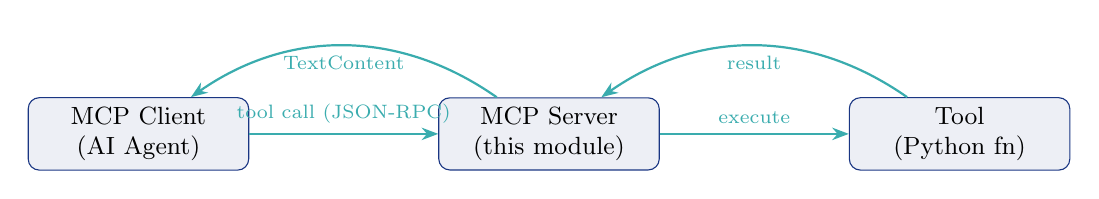
\begin{tikzpicture}[
  node distance=1.8cm,
  box/.style={draw=SesameNavy, fill=SesameNavy!8, rounded corners=4pt,
              minimum width=2.8cm, minimum height=0.8cm, font=\small,
              align=center},
  arr/.style={-{Stealth[length=6pt]}, thick, color=SesameTeal},
]
  \node[box] (client) {MCP Client\\(AI Agent)};
  \node[box, right=2.4cm of client] (server) {MCP Server\\(this module)};
  \node[box, right=2.4cm of server] (tool) {Tool\\(Python fn)};
  \draw[arr] (client) -- node[above,font=\scriptsize]{tool call (JSON-RPC)} (server);
  \draw[arr] (server) -- node[above,font=\scriptsize]{execute} (tool);
  \draw[arr] (tool) to[bend right=35] node[below,font=\scriptsize]{result} (server);
  \draw[arr] (server) to[bend right=35] node[below,font=\scriptsize]{TextContent} (client);
\end{tikzpicture}
\end{center}

\subsection{FastMCP Tool Definition}

FastMCP lets you define a tool with a single decorator. The type annotations
automatically generate the JSON Schema that the LLM uses to fill in arguments.

\begin{lstlisting}[language=Python, caption={FastMCP tool — automatic schema from type hints}]
from mcp.server.fastmcp import FastMCP
from typing import Annotated

mcp = FastMCP(name="calculator-server")

@mcp.tool(description="Evaluate a mathematical expression safely.")
def calculate(
    expression: Annotated[str, "Math expression, e.g. 'sqrt(144) + 2**10'"],
) -> dict:
    """Uses sympy.sympify -- no eval() for security."""
    _validate_expression(expression)          # whitelist check
    parsed = sp.sympify(expression, evaluate=True)
    return {"input": expression, "result": float(parsed.evalf())}
\end{lstlisting}

\subsection{Security: No \texttt{eval()}}

\begin{warnbox}
\textbf{Critical:} Never use Python's built-in \texttt{eval()} on user input.
It can execute arbitrary code. This lab uses \texttt{sympy.sympify()} combined
with a regex whitelist that only allows digits, operators, parentheses, and
Latin letters. Anything with quotes, brackets \texttt{[]}, or special characters
is rejected before reaching SymPy.
\end{warnbox}

\begin{lstlisting}[language=Python, caption={Security validation}]
import re

_SAFE_CHARS = re.compile(r"^[\d\s\+\-\*/\^\(\)\.,a-zA-Z_=<>!]+$")

def _validate_expression(expr: str) -> None:
    if not expr or not expr.strip():
        raise ValueError("Expression must not be empty.")
    if not _SAFE_CHARS.match(expr):
        raise ValueError("Expression contains disallowed characters.")
\end{lstlisting}

\subsection{Available Calculator Tools}

\begin{center}
\begin{tabularx}{\linewidth}{lXl}
\toprule
\textbf{Tool} & \textbf{Description} & \textbf{Library} \\
\midrule
\texttt{calculate}     & Evaluate arithmetic / trig / log expression & SymPy \\
\texttt{solve\_equation} & Solve algebraic equation for variable & SymPy \\
\texttt{metrics}       & Descriptive statistics (mean, std, quartiles) & NumPy \\
\texttt{unit\_convert} & Physical unit conversion (km/h $\rightarrow$ m/s, etc.) & Pint \\
\texttt{matrix\_ops}   & Add, multiply, determinant, inverse & NumPy \\
\bottomrule
\end{tabularx}
\end{center}

% ─────────────────────────────────────────────────────────────────────────────
\newpage
\section{Notes MCP Server}
% ─────────────────────────────────────────────────────────────────────────────

\subsection{Purpose}

The Notes server demonstrates that MCP is not limited to computation — any
structured service (key-value store, search index, document database) can be
wrapped as an MCP tool server, enabling AI agents to \emph{remember} information
across conversation turns.

\subsection{NoteStore Architecture}

\begin{lstlisting}[language=Python, caption={In-memory NoteStore}]
class NoteStore:
    def __init__(self) -> None:
        self._notes: dict[str, dict] = {}   # note_id -> note dict

    def create(self, title: str, body: str,
               tags: list[str] | None = None) -> dict:
        note_id = str(uuid.uuid4())[:8]
        note = {"id": note_id, "title": title.strip(),
                "body": body.strip(), "tags": tags or [],
                "created_at": ..., "updated_at": ...}
        self._notes[note_id] = note
        return note

    def search(self, query: str) -> list[dict]:
        q = query.lower()
        return [n for n in self._notes.values()
                if q in n["title"].lower()
                or q in n["body"].lower()
                or any(q in t.lower() for t in n["tags"])]
\end{lstlisting}

\subsection{Tools Exposed}

\begin{center}
\begin{tabularx}{\linewidth}{lX}
\toprule
\textbf{Tool} & \textbf{Description} \\
\midrule
\texttt{create\_note}  & Add a new note (title, body, optional tags) \\
\texttt{get\_note}     & Retrieve full note by 8-char ID \\
\texttt{list\_notes}   & List all notes (summaries, no body) \\
\texttt{search\_notes} & Full-text search across title, body, tags \\
\texttt{update\_note}  & Edit title and/or body of existing note \\
\texttt{delete\_note}  & Remove a note by ID \\
\bottomrule
\end{tabularx}
\end{center}

\begin{infobox}
\textbf{In-memory vs. persistent:} The NoteStore resets on server restart.
For persistence, replace the internal \texttt{dict} with a SQLite backend
or Django ORM queryset. The tool interface stays identical — no agent changes needed.
\end{infobox}

% ─────────────────────────────────────────────────────────────────────────────
\newpage
\section{Groq LLM Integration (Strategy Pattern)}
% ─────────────────────────────────────────────────────────────────────────────

\subsection{The Strategy Pattern}

The LLM layer is designed with the \textbf{Strategy pattern}: an abstract
\texttt{LLMProvider} defines the interface; \texttt{GroqProvider} is the
concrete implementation. Swapping to OpenAI or a local Ollama model requires
only changing one environment variable, not the agent code.

\begin{lstlisting}[language=Python, caption={Abstract LLM provider (Strategy interface)}]
from abc import ABC, abstractmethod
from dataclasses import dataclass

@dataclass
class LLMMessage:
    role: str          # "system" | "user" | "assistant" | "tool"
    content: str
    tool_call_id: str | None = None
    tool_calls: list[dict] | None = None

@dataclass
class LLMResponse:
    content: str | None
    tool_calls: list[dict]   # OpenAI function-calling format
    finish_reason: str = "stop"

class LLMProvider(ABC):
    @abstractmethod
    async def chat_with_tools(
        self, messages: list[LLMMessage], tools: list[dict], **kwargs
    ) -> LLMResponse: ...

    @property
    @abstractmethod
    def model_name(self) -> str: ...
\end{lstlisting}

\subsection{Groq Provider with Retry Logic}

\begin{lstlisting}[language=Python, caption={GroqProvider with exponential back-off}]
import backoff
from groq import AsyncGroq

class GroqProvider(LLMProvider):
    def __init__(self, api_key: str, model: str = "llama-3.3-70b-versatile",
                 timeout: float = 30.0, max_retries: int = 3):
        self._client = AsyncGroq(api_key=api_key, timeout=timeout)
        self._model  = model
        self._max_retries = max_retries

    async def chat_with_tools(self, messages, tools, **kwargs) -> LLMResponse:
        @backoff.on_exception(backoff.expo, Exception,
                              max_tries=self._max_retries,
                              giveup=lambda e: not _is_retryable(e))
        async def _call():
            resp = await self._client.chat.completions.create(
                model=self._model,
                messages=[m.__dict__ for m in messages],
                tools=tools or None,
            )
            choice = resp.choices[0]
            return LLMResponse(
                content=choice.message.content,
                tool_calls=[tc.__dict__ for tc in (choice.message.tool_calls or [])],
                finish_reason=choice.finish_reason,
            )
        return await _call()
\end{lstlisting}

% ─────────────────────────────────────────────────────────────────────────────
\newpage
\section{AI Agents and the ReAct Loop}
% ─────────────────────────────────────────────────────────────────────────────

\subsection{What is ReAct?}

\textbf{ReAct} (\textbf{Re}ason + \textbf{Act}) is an agent architecture where the LLM
alternates between:
\begin{enumerate}
  \item \textbf{Reason} — the LLM thinks about which tool to call (or gives a final answer).
  \item \textbf{Act} — the agent executes the tool and appends the result to the conversation.
  \item \textbf{Observe} — the tool result is fed back to the LLM.
\end{enumerate}
This loop repeats until the LLM produces a text answer (no tool call).

\begin{center}
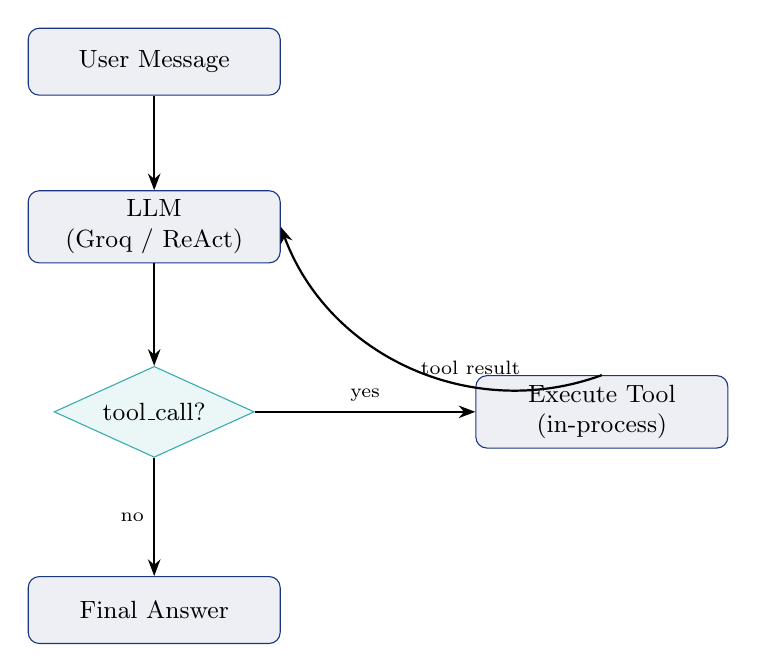
\begin{tikzpicture}[
  node distance=1.5cm and 2.5cm,
  box/.style={draw=SesameNavy, fill=SesameNavy!8, rounded corners=4pt,
              minimum width=3.2cm, minimum height=0.85cm, font=\small,
              align=center},
  decision/.style={draw=SesameTeal, fill=SesameTeal!10, diamond, aspect=2.2,
                   font=\small, align=center},
  arr/.style={-{Stealth[length=6pt]}, thick},
]
  \node[box] (user) {User Message};
  \node[box, below=1.2cm of user] (llm) {LLM\\(Groq / ReAct)};
  \node[decision, below=1.3cm of llm] (decide) {tool\_call?};
  \node[box, right=2.8cm of decide] (tool) {Execute Tool\\(in-process)};
  \node[box, below=1.5cm of decide] (answer) {Final Answer};

  \draw[arr] (user) -- (llm);
  \draw[arr] (llm) -- (decide);
  \draw[arr] (decide) -- node[above,font=\scriptsize]{yes} (tool);
  \draw[arr] (tool.north) to[bend left=45] node[right,font=\scriptsize]{tool result} (llm.east);
  \draw[arr] (decide) -- node[left,font=\scriptsize]{no} (answer);
\end{tikzpicture}
\end{center}

\subsection{BaseAgent Implementation}

\begin{lstlisting}[language=Python, caption={ReAct loop in BaseAgent.run()}]
async def run(self, user_message: str) -> AgentResponse:
    messages = [
        LLMMessage(role="system", content=self.system_prompt),
        LLMMessage(role="user",   content=user_message),
    ]
    tool_calls_made = []

    for step in range(1, self._max_steps + 1):
        resp = await self._llm.chat_with_tools(messages, self._tool_definitions())

        # -- No tool call -> LLM gave final answer --------------------------
        if not resp.tool_calls:
            return AgentResponse(answer=resp.content,
                                 tool_calls_made=tool_calls_made)

        # -- Tool call(s) requested -----------------------------------------
        messages.append(LLMMessage(role="assistant",
                                   content=resp.content or "",
                                   tool_calls=resp.tool_calls))

        for tc in resp.tool_calls:
            fn_name = tc["function"]["name"]
            args    = json.loads(tc["function"]["arguments"])
            result  = await self._execute_tool(fn_name, args)
            tool_calls_made.append(fn_name)
            messages.append(LLMMessage(role="tool", content=result,
                                       tool_call_id=tc["id"]))

    # Max steps exceeded
    return AgentResponse(answer="Max steps reached.", error="max_steps_exceeded",
                         tool_calls_made=tool_calls_made)
\end{lstlisting}

\subsection{CalculatorAgent Tool Definitions}

\begin{lstlisting}[language=Python, caption={OpenAI function-calling format for tool definitions}]
_TOOLS = [
  {
    "type": "function",
    "function": {
      "name": "calculate",
      "description": "Evaluate a math expression. E.g.: sqrt(144) + log(E**2)",
      "parameters": {
        "type": "object",
        "properties": {
          "expression": {"type": "string",
                         "description": "Expression to evaluate"}
        },
        "required": ["expression"]
      }
    }
  },
  # ... solve_equation, metrics, unit_convert, matrix_ops
]
\end{lstlisting}

% ─────────────────────────────────────────────────────────────────────────────
\newpage
\section{A2A Protocol}
% ─────────────────────────────────────────────────────────────────────────────

\subsection{What is A2A?}

\textbf{Agent-to-Agent (A2A)} communication enables multiple specialised agents to
collaborate: one agent decomposes a task and delegates sub-tasks to other agents
via a structured message envelope.

\subsection{A2AMessage Schema}

\begin{lstlisting}[language=Python, caption={A2AMessage dataclass}]
@dataclass
class A2AMessage:
    from_agent:   str               # sender agent name
    to_agent:     str               # target agent name
    content:      dict[str, Any]    # {"message": "...", ...}
    message_type: MessageType = MessageType.TASK
    task_id:      str         = field(default_factory=lambda: uuid.uuid4()[:12])
    state:        TaskState   = TaskState.SUBMITTED
    timestamp:    str         = field(default_factory=_now_iso)
    parent_id:    str | None  = None
\end{lstlisting}

\subsection{Task States}

\begin{center}
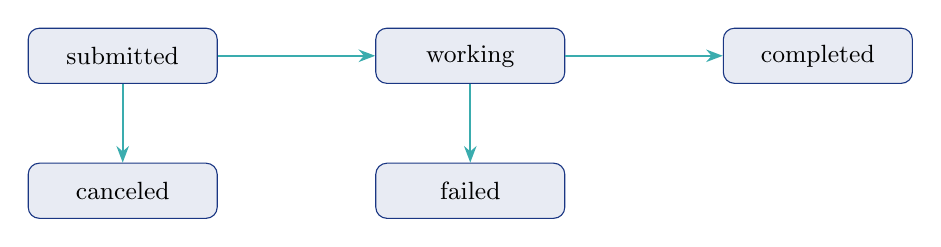
\begin{tikzpicture}[
  state/.style={draw=SesameNavy, fill=SesameNavy!10, rounded corners=4pt,
                minimum width=2.4cm, minimum height=0.7cm, font=\small},
  arr/.style={-{Stealth[length=6pt]}, thick, color=SesameTeal},
  node distance=1.4cm and 2cm,
]
  \node[state] (sub)  {submitted};
  \node[state, right=2cm of sub]  (work) {working};
  \node[state, right=2cm of work] (done) {completed};
  \node[state, below=1cm of work] (fail) {failed};
  \node[state, below=1cm of sub]  (can)  {canceled};

  \draw[arr] (sub)  -- (work);
  \draw[arr] (work) -- (done);
  \draw[arr] (work) -- (fail);
  \draw[arr] (sub)  -- (can);
\end{tikzpicture}
\end{center}

\subsection{AgentRegistry (Singleton)}

\begin{lstlisting}[language=Python, caption={Singleton registry}]
class AgentRegistry:
    _instance: "AgentRegistry | None" = None

    def __new__(cls) -> "AgentRegistry":
        if cls._instance is None:
            cls._instance = super().__new__(cls)
            cls._instance._agents = {}
            cls._instance._cards  = {}
        return cls._instance

    def register(self, agent: BaseAgent, card: AgentCard) -> None:
        self._agents[card.name] = agent
        self._cards[card.name]  = card

    def find_by_capability(self, capability: str) -> list[str]:
        return [name for name, card in self._cards.items()
                if capability in card.capabilities]
\end{lstlisting}

\subsection{TaskRouter (Keyword Routing)}

\begin{lstlisting}[language=Python, caption={Keyword-based routing rules}]
_ROUTING_RULES = [
    (re.compile(r"calculat|arith|math|equat|solv|sqrt|matrix|statistic"
                r"|metric|mean|median|unit convert|km/h", re.I), "math"),
    (re.compile(r"\bnote\b|remember|store.*note|find.*note"
                r"|recall|my note|write down|save this", re.I), "notes"),
]

def _infer_capability(self, text: str) -> str | None:
    for pattern, capability in _ROUTING_RULES:
        if pattern.search(text):
            return capability
    return None  # coordinator decides
\end{lstlisting}

% ─────────────────────────────────────────────────────────────────────────────
\newpage
\section{Django Async Views}
% ─────────────────────────────────────────────────────────────────────────────

\subsection{Async View Pattern}

Django 4.1+ supports native \texttt{async def} views. This lab uses
\textbf{ASGI + Uvicorn} to serve requests concurrently without blocking
the event loop during I/O.

\begin{lstlisting}[language=Python, caption={Async view with sync ORM wrapper}]
from asgiref.sync import sync_to_async
from django.http import JsonResponse

async def api_calculate(request: HttpRequest) -> JsonResponse:
    """Direct MCP calculator tool call (no LLM)."""
    body = json.loads(request.body or "{}")
    tool   = body.get("tool", "calculate")
    params = body.get("params", {})

    # -- Dispatch to MCP tool (in-process, fast) ----------------------------
    result = calculate(expression=params.get("expression", ""))

    # -- ORM call must be wrapped with sync_to_async ------------------------
    await sync_to_async(CalculationLog.objects.create)(
        expression=json.dumps(params),
        result=json.dumps(result),
        tool_used=tool,
        success="error" not in result,
    )
    return JsonResponse({"tool": tool, "result": result})
\end{lstlisting}

\subsection{Why \texttt{sync\_to\_async}?}

Django's ORM is synchronous (it uses thread-local database connections).
Calling ORM methods directly from an \texttt{async def} view would either
block the event loop or raise a \texttt{SynchronousOnlyOperation} error.
\texttt{sync\_to\_async} wraps the call in a thread pool executor so the
event loop stays unblocked.

\begin{center}
\begin{tabularx}{\linewidth}{lXX}
\toprule
\textbf{Aspect}        & \textbf{WSGI (old)}       & \textbf{ASGI (this lab)} \\
\midrule
Concurrency            & 1 request per thread      & Multiple requests in one thread \\
Waiting on I/O         & Thread blocks             & Event loop switches tasks \\
Groq API call          & Blocks thread             & \texttt{await} yields to loop \\
Django ORM             & Direct call               & \texttt{sync\_to\_async} wrapper \\
Server                 & Gunicorn                  & Uvicorn \\
SSE / WebSockets       & Not native                & Native \\
\bottomrule
\end{tabularx}
\end{center}

\subsection{REST API Reference}

\begin{center}
\begin{tabularx}{\linewidth}{llX}
\toprule
\textbf{Method} & \textbf{URL} & \textbf{Description} \\
\midrule
POST & \texttt{/api/calculate/}    & Direct MCP tool call (no LLM) \\
POST & \texttt{/api/agent/chat/}   & Agent chat with ReAct loop \\
POST & \texttt{/api/a2a/delegate/} & A2A task delegation \\
GET  & \texttt{/api/agents/}       & List registered agent cards \\
GET  & \texttt{/.well-known/agent.json} & A2A coordinator card \\
\bottomrule
\end{tabularx}
\end{center}

% ─────────────────────────────────────────────────────────────────────────────
\newpage
\section{Testing Strategy}
% ─────────────────────────────────────────────────────────────────────────────

\subsection{Test Pyramid}

\begin{center}
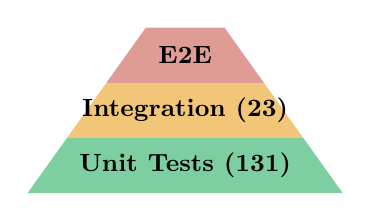
\begin{tikzpicture}
  \fill[SesameGreen!60]  (0,0) -- (4,0) -- (3.5,0.7) -- (0.5,0.7) -- cycle;
  \fill[SesameGold!60]   (0.5,0.7) -- (3.5,0.7) -- (3.0,1.4) -- (1.0,1.4) -- cycle;
  \fill[SesameRed!50]    (1.0,1.4) -- (3.0,1.4) -- (2.5,2.1) -- (1.5,2.1) -- cycle;
  \node[font=\small\bfseries] at (2,0.35) {Unit Tests (131)};
  \node[font=\small\bfseries] at (2,1.05) {Integration (23)};
  \node[font=\small\bfseries] at (2,1.75) {E2E};
\end{tikzpicture}
\end{center}

\subsection{Unit Tests}

\begin{itemize}
  \item \textbf{test\_calculator.py} (35 tests) — each tool function individually.
    Security: blocked expressions with quotes, brackets.
  \item \textbf{test\_notes.py} (36 tests) — NoteStore CRUD, search, update, delete.
  \item \textbf{test\_a2a.py} (41 tests) — A2AMessage round-trips,
    AgentRegistry singleton, TaskRouter keyword routing.
  \item \textbf{test\_agents.py} (19 tests) — ReAct loop with ScriptedLLMProvider
    (no Groq key needed).
\end{itemize}

\subsection{Key Testing Pattern: Scripted LLM}

\begin{lstlisting}[language=Python, caption={Mock LLM for deterministic agent tests}]
class ScriptedLLMProvider(LLMProvider):
    """Replay fixed LLMResponse objects. No Groq API required."""

    def __init__(self, responses: list[LLMResponse]):
        self._responses = responses
        self._index = 0

    async def chat_with_tools(self, messages, tools, **kwargs) -> LLMResponse:
        resp = self._responses[self._index]
        self._index += 1
        return resp

    @property
    def model_name(self) -> str:
        return "fake-llm"

# Usage:
provider = ScriptedLLMProvider([
    LLMResponse(content=None,
                tool_calls=[{"id": "c1", "function":
                             {"name": "calculate",
                              "arguments": '{"expression": "sqrt(144)"}'}}]),
    LLMResponse(content="The square root of 144 is 12.", tool_calls=[]),
])
agent = CalculatorAgent(llm=provider)
result = await agent.run("What is sqrt(144)?")
assert result.answer == "The square root of 144 is 12."
assert "calculate" in result.tool_calls_made
\end{lstlisting}

\subsection{Running the Tests}

\begin{lstlisting}[language=bash, caption={Running the test suite}]
# All tests (154 total)
pytest

# Single test file
pytest mcp_engine/tests/test_calculator.py -v

# Only fast unit tests (skip views)
pytest mcp_engine/tests/ --ignore=mcp_engine/tests/test_views.py

# With coverage
pip install pytest-cov
pytest --cov=mcp_engine --cov-report=html
open htmlcov/index.html
\end{lstlisting}

% ─────────────────────────────────────────────────────────────────────────────
\newpage
\section{Docker Deployment}
% ─────────────────────────────────────────────────────────────────────────────

\subsection{Dockerfile Overview}

The Dockerfile uses a \textbf{multi-stage build}:

\begin{enumerate}
  \item \textbf{Stage 1 (builder):} installs all Python packages.
  \item \textbf{Stage 2 (runtime):} copies only the installed packages,
    not the build tools — resulting in a smaller, more secure final image.
\end{enumerate}

\begin{lstlisting}[language=bash, caption={Docker usage}]
# 1. Fill in the API key
cp .env.example .env
# Edit .env: GROQ_API_KEY=gsk_...

# 2. Build and start
docker compose up --build

# 3. The app is now running at http://localhost:8000/

# 4. View logs
docker compose logs -f web

# 5. Stop
docker compose down
\end{lstlisting}

\subsection{Key Docker Concepts Used}

\begin{center}
\begin{tabularx}{\linewidth}{lX}
\toprule
\textbf{Concept} & \textbf{Implementation} \\
\midrule
Multi-stage build  & Lean runtime image; no compiler tools in production \\
Non-root user      & \texttt{appuser:appgroup (UID 1001)} \\
Volume persistence & SQLite database survives container restarts \\
Health check       & HTTP GET \texttt{/} every 30s; 3 retries \\
Resource limits    & 1 CPU, 512 MB RAM (adjustable) \\
Env var secrets    & GROQ\_API\_KEY from \texttt{.env} (never baked in) \\
\bottomrule
\end{tabularx}
\end{center}

\begin{warnbox}
\textbf{Production checklist:}
Set \texttt{DJANGO\_DEBUG=False}, \texttt{DJANGO\_SECRET\_KEY} to a random
256-bit string, and \texttt{DJANGO\_ALLOWED\_HOSTS} to your domain name before
deploying to the internet. Change the default SQLite backend to PostgreSQL
for multi-process deployments.
\end{warnbox}

% ─────────────────────────────────────────────────────────────────────────────
\newpage
\section{Exercises}
% ─────────────────────────────────────────────────────────────────────────────

\subsection{Beginner}

\begin{enumerate}[leftmargin=*, label=\textbf{B\arabic*.}]
  \item Open \texttt{http://localhost:8000/calculator/} and call the
        \texttt{calculate} tool with the expression
        \texttt{sin(pi/6) + cos(pi/3)}. What is the result? Explain why.

  \item Use the Notes UI to create three notes about Django topics.
        Then search for one of them by keyword. Screenshot the result.

  \item In the A2A Demo, use the ``Coordinator $\rightarrow$ NoteBot'' scenario button.
        Describe what you see in the A2A Task Log. Which agent was selected?
        Why?

  \item Open \texttt{/.well-known/agent.json} in a browser.
        What information does it expose? Why is this URL standardised?
\end{enumerate}

\subsection{Intermediate}

\begin{enumerate}[leftmargin=*, label=\textbf{I\arabic*.}]
  \item \textbf{Add a new MCP tool.} Add a \texttt{prime\_factors} tool to
        \texttt{calculator.py} that returns the prime factorisation of a
        positive integer. Use \texttt{sympy.factorint()}.
        Write at least 3 pytest tests for it.

  \item \textbf{Extend the router.} Add a routing rule that matches questions
        about physics units (e.g. "convert joules to calories") and routes
        them to the \texttt{calculator\_agent}.
        Write a parametrised test for the new rule.

  \item \textbf{Persistent notes.} Replace the \texttt{NoteStore} dictionary
        with a Django model-backed store. Implement \texttt{create},
        \texttt{get}, \texttt{search}, and \texttt{delete} using the ORM.
        Wrap ORM calls with \texttt{sync\_to\_async} if called from an async
        context.

  \item \textbf{Rate-limit display.} Add a \texttt{/history/} UI counter
        showing how many Groq API calls were made in the last 60 seconds.
        Use the \texttt{AgentSession.created\_at} field.
\end{enumerate}

\subsection{Advanced}

\begin{enumerate}[leftmargin=*, label=\textbf{A\arabic*.}]
  \item \textbf{Add a third agent} — a \texttt{WeatherAgent} that calls
        a free weather API (e.g. Open-Meteo, no key needed).
        Register it in the orchestrator and add routing keywords
        (\texttt{"weather"}, \texttt{"temperature"}, \texttt{"forecast"}).

  \item \textbf{Streaming response.} Replace the \texttt{api\_agent\_chat}
        endpoint with a Server-Sent Events (SSE) streaming endpoint that
        sends each ReAct step as an event. Update the JS chat UI to render
        tool-call events in real time as they arrive.

  \item \textbf{Hierarchical A2A.} Implement a \texttt{PlannerAgent} that
        receives a complex multi-part question (e.g. "What is the mean of
        [1,2,3] and save the result as a note?"), decomposes it into two
        sub-tasks, delegates each to the appropriate agent via \texttt{A2AMessage},
        and then combines the results into a single final answer.

  \item \textbf{OpenAI provider.} Implement \texttt{OpenAIProvider} that
        satisfies the \texttt{LLMProvider} interface. Make the provider
        selectable by setting \texttt{LLM\_BACKEND=openai} in \texttt{.env}.
        The agents must work without any code changes.
\end{enumerate}

% ─────────────────────────────────────────────────────────────────────────────
\newpage
\section{Architecture Summary}
% ─────────────────────────────────────────────────────────────────────────────

\subsection{Full System Diagram}

\begin{center}
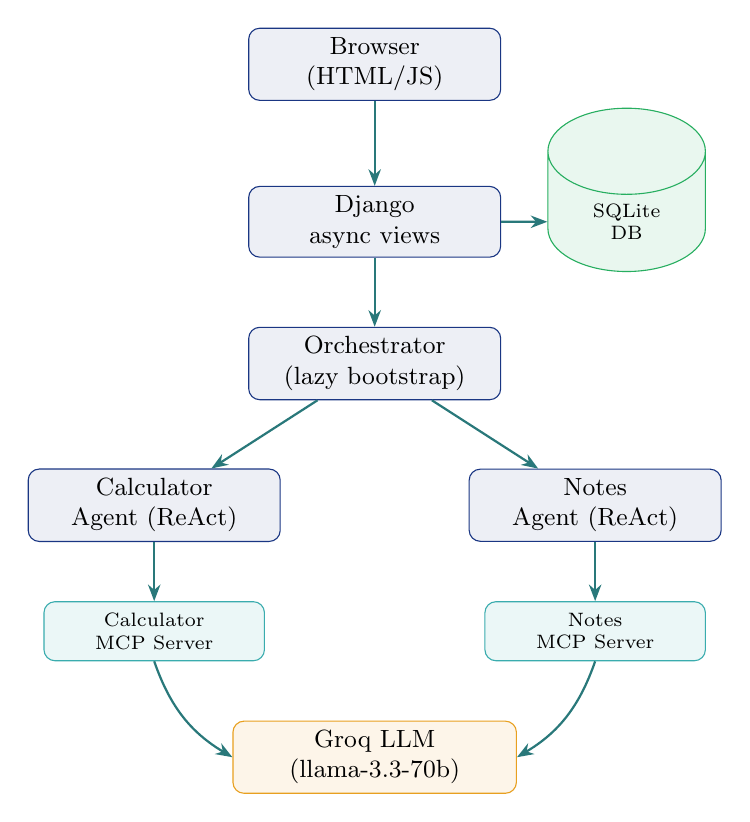
\begin{tikzpicture}[
  box/.style={draw=SesameNavy, fill=SesameNavy!8, rounded corners=4pt,
              minimum width=3.2cm, minimum height=0.85cm, font=\small, align=center},
  mcp/.style={draw=SesameTeal, fill=SesameTeal!10, rounded corners=4pt,
              minimum width=2.8cm, minimum height=0.75cm, font=\scriptsize, align=center},
  llm/.style={draw=SesameGold, fill=SesameGold!10, rounded corners=4pt,
              minimum width=3.6cm, minimum height=0.8cm, font=\small, align=center},
  db/.style={draw=SesameGreen, fill=SesameGreen!10, cylinder,
             shape border rotate=90, minimum width=2cm, minimum height=0.85cm,
             font=\scriptsize, align=center},
  arr/.style={-{Stealth[length=6pt]}, thick, color=SesameTeal!70!black},
]
  %--- Layer 1: Browser (top-centre) ---
  \node[box] at (0,0) (browser) {Browser\\(HTML/JS)};

  %--- Layer 2: Django views + SQLite (right) ---
  \node[box] at (0,-2)   (views) {Django\\async views};
  \node[db]  at (3.2,-2) (db)    {SQLite\\DB};

  %--- Layer 3: Orchestrator ---
  \node[box] at (0,-3.8) (orch) {Orchestrator\\(lazy bootstrap)};

  %--- Layer 4: Agents (left / right) ---
  \node[box] at (-2.8,-5.6) (calc) {Calculator\\Agent (ReAct)};
  \node[box] at ( 2.8,-5.6) (note) {Notes\\Agent (ReAct)};

  %--- Layer 5: MCP Servers ---
  \node[mcp] at (-2.8,-7.2) (calcmcp) {Calculator\\MCP Server};
  \node[mcp] at ( 2.8,-7.2) (notemcp) {Notes\\MCP Server};

  %--- Layer 6: Groq LLM (bottom-centre) ---
  \node[llm] at (0,-8.8) (groq) {Groq LLM\\(llama-3.3-70b)};

  %--- Arrows ---
  \draw[arr] (browser)        -- (views);
  \draw[arr] (views)          -- (db);
  \draw[arr] (views)          -- (orch);
  \draw[arr] (orch)           -- (calc);
  \draw[arr] (orch)           -- (note);
  \draw[arr] (calc)           -- (calcmcp);
  \draw[arr] (note)           -- (notemcp);
  \draw[arr] (calcmcp.south)  to[bend right=20] (groq.west);
  \draw[arr] (notemcp.south)  to[bend left=20]  (groq.east);
\end{tikzpicture}
\end{center}

\subsection{Design Patterns Used}

\begin{center}
\begin{tabularx}{\linewidth}{lXl}
\toprule
\textbf{Pattern} & \textbf{Where} & \textbf{Benefit} \\
\midrule
Strategy         & LLMProvider / GroqProvider      & Swap LLM without touching agents \\
Singleton        & AgentRegistry                   & One global agent directory \\
Template Method  & BaseAgent.run()                 & ReAct loop shared by all agents \\
Lazy Init        & Orchestrator \_bootstrap()      & No startup cost if unused \\
Registry         & AgentRegistry                   & Decouple agents from coordinator \\
\bottomrule
\end{tabularx}
\end{center}

\subsection{Key Takeaways}

\begin{successbox}
\begin{enumerate}[leftmargin=*, itemsep=2pt]
  \item \textbf{MCP} standardises how AI models call external tools — the LLM never
        sees raw Python code, only a JSON schema.
  \item \textbf{ReAct} is more reliable than one-shot prompting for tasks requiring
        multi-step reasoning and tool use.
  \item \textbf{A2A} enables specialisation: each agent is an expert; the coordinator
        routes rather than does everything itself.
  \item \textbf{Async Django} (ASGI + Uvicorn) handles I/O-bound work (LLM API calls)
        efficiently without spawning new threads.
  \item \textbf{Never \texttt{eval()}.} Use \texttt{sympy.sympify()} + a character
        whitelist for safe user-provided math expressions.
  \item \textbf{Test without secrets.} The \texttt{ScriptedLLMProvider} pattern lets
        you fully test agent logic without a live API key.
\end{enumerate}
\end{successbox}

\vspace{2cm}
\begin{center}
{\color{SesameNavy}\rule{0.5\linewidth}{1pt}}\\[0.5em]
{\small\color{gray}AI Agent Lab · Sesame University 2025--2026 · MCP · A2A · Groq · Django}
\end{center}

\end{document}
